% Auriga theme
% https://github.com/anishathalye/auriga

\documentclass[12pt,aspectratio=169]{beamer}
\usepackage{pgfpages}
\usepackage{fancyvrb}
\usepackage{tikz}
\usepackage{pgfplots}
\usepackage{multirow}
\usepackage{graphicx}
\graphicspath{ {./img/} }

\ifnotes
\setbeamertemplate{note page}[plain]
\setbeameroption{show notes on second screen=right}
\fi

\usetheme{auriga}
\usecolortheme{auriga}

% define some colors for a consistent theme across slides
\definecolor{red}{RGB}{181, 23, 0}
\definecolor{blue}{RGB}{0, 118, 186}
\definecolor{gray}{RGB}{146, 146, 146}
\definecolor{turq}{RGB}{75,136,162}
\definecolor{sred}{RGB}{187,10,33}
\definecolor{violet}{RGB}{53,20,49}
\definecolor{salmon}{RGB}{240,100,73}

\title{The {\color{sred}Diversity}-{\color{turq}Bandwidth} Trade-off}

\author{Sinan Aral \and Marshall Van Alstyne}

% \author{Sinan Aral \inst{1} \and Marshall Van Alstyne \inst{2}}

% \institute[shortinst]{\inst{1} New York University \samelineand \inst{2} Boston University}

\begin{document}

{
  % rather than use the frame options [noframenumbering,plain], we make the
  % color match, so that the indicated page numbers match PDF page numbers
  \setbeamercolor{page number in head/foot}{fg=background canvas.bg}
  \begin{frame}
    \titlepage
    {\color{gray}{By: Adarsh Mathew}}
  \end{frame}
}

\begin{frame}{{\color{violet} Key Questions}}

  \begin{itemize}
    \item Where do we find {\color{salmon}Novel} Information? 
    \item At what rate do we receive {\color{salmon}novelty} from our different social contacts?
    \item Is there empirical evidence of a trade-off between \underline{Network {\color{sred}Diversity}} and \underline{Channel {\color{turq}Bandwidth}}?
  \end{itemize}

  % \begin{center}
     
    
      
    
    
  % \end{center}

  % \vspace{2ex}
  % \begin{center}
  %   \scriptsize (Local information is redundant $\rightarrow$ Far ties have novel information)
  % \end{center}

  % \vspace{1ex}
  % \begin{itemize}
  % 	\item Implication: Greater network diversity is associated with lower channel bandwidth
  % 	\item Limitation: Content-agnostic
  % \end{itemize}

\end{frame}

\begin{frame}{{\color{violet}Theory 1: {\color{salmon}Novelty} via {\color{sred}Diverse} Ties}}

  \begin{center}
    Structurally {\color{sred}diverse} networks -- low in cohesion and structural equivalence and rich in structural holes -- provide access to diverse, {\color{salmon}novel} information
  \end{center}

  \vspace{2ex}
  \begin{center}
    \scriptsize (Local information is redundant $\rightarrow$ Far ties have novel information)
  \end{center}

  % \vspace{1ex}
  % \begin{itemize}
  % 	\item Implication: Greater network diversity is associated with lower channel bandwidth
  % 	\item Limitation: Content-agnostic
  % \end{itemize}

\end{frame}

\begin{frame}{{\color{violet} Limitations of Structural Holes Theory}}

  \begin{itemize}
    \item Content-agnostic
    \begin{itemize}
      \item Role of information complexity
      \item How often does the information get updated
    \end{itemize}
    \item `Information exchange is fundamentally a \underline{social process} and knowledge transfer a discretionary activity'
  \end{itemize}

\end{frame}

\begin{frame}{{\color{violet}Theory 2: {\color{salmon}Novelty} via high {\color{blue}Bandwidth} Ties}}

  \begin{center}
    Greater channel {\color{blue}bandwidth} in high-cohesion ties should increase access to {\color{salmon}novel} information
  \end{center}

  \vspace{2ex}
  \begin{center}
    \scriptsize (Social Processes: Social Capital, Transactive Memory, Search Transfer, Knowledge Creation, Homophily)
  \end{center}


  % \begin{itemize}
  % 	\item Social Capital: Low-bandwidth networks are opportunistic
  % 	\item Transactive Memory: Familiarity of alter's expertise inspires greater exchange
  % 	\item Search Transfer: Complex information requires high-bandwidth 
  % 	\item Knowledge Creation: Requires repeated interaction => high-bandwidth channels
  % 	\item Homophily: Deeper engagement creates mutual areas of interest  
  % \end{itemize}

\end{frame}

\begin{frame}{{\color{violet}Theory 2: {\color{salmon}Novelty} via high {\color{blue}Bandwidth} Ties}}

  \begin{center}
    Greater channel {\color{blue}bandwidth} in high-cohesion ties should increase access to {\color{salmon}novel} information
  \end{center}

  \vspace{2ex}
  \begin{center}
    \scriptsize (Social Processes: Social Capital, Transactive Memory, Search Transfer, Knowledge Creation, Homophily)
  \end{center}


  % \begin{itemize}
  % 	\item Social Capital: Low-bandwidth networks are opportunistic
  % 	\item Transactive Memory: Familiarity of alter's expertise inspires greater exchange
  % 	\item Search Transfer: Complex information requires high-bandwidth 
  % 	\item Knowledge Creation: Requires repeated interaction => high-bandwidth channels
  % 	\item Homophily: Deeper engagement creates mutual areas of interest  
  % \end{itemize}

\end{frame}

\begin{frame}{\color{violet} Content Considerations of the Trade-off}

  \begin{figure}
    \centering
    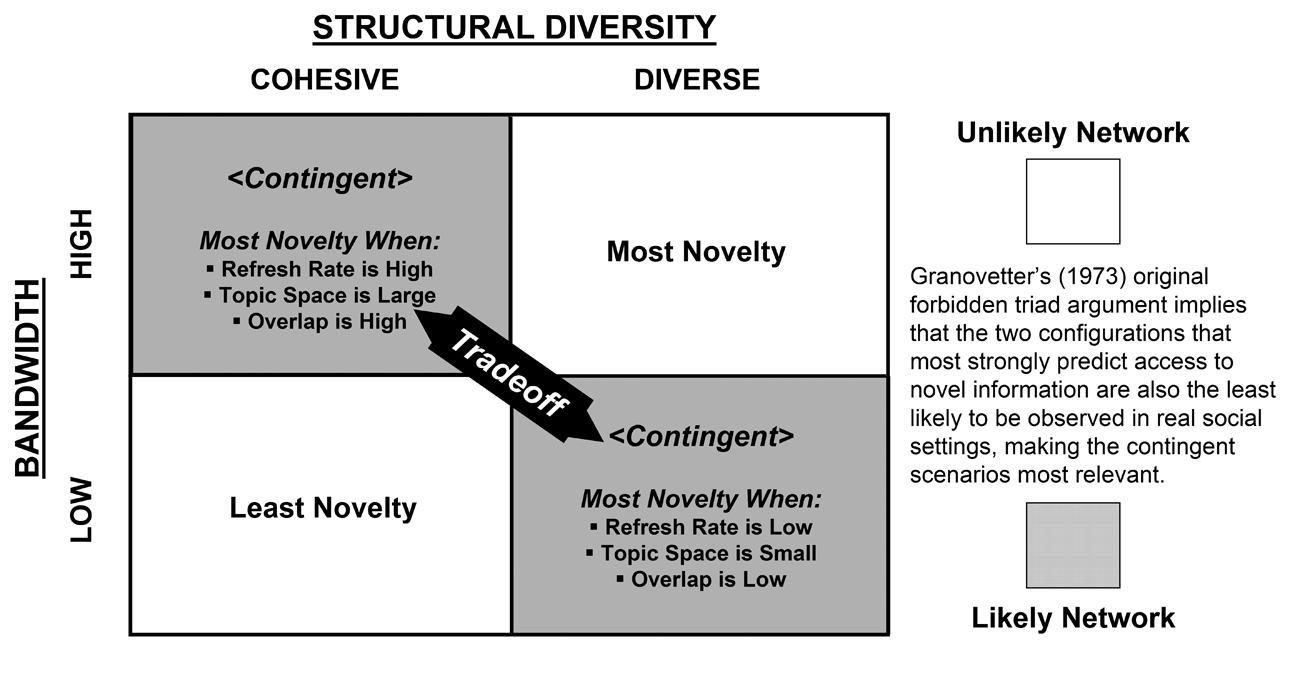
\includegraphics[width=\linewidth]{tbl_bandwidth-diversity.png}
    \caption{Diversity-Bandwidth Trade-off}
  \end{figure}


\end{frame}

\begin{frame}{\color{violet} Model Hypotheses}

% Please add the following required packages to your document preamble:
% \usepackage{graphicx}
\begin{table}[]
\resizebox{\textwidth}{!}{%
\begin{tabular}{|p{0.07\linewidth}|p{0.93\linewidth}|}
\hline
    & \textbf{Hypothesized Relationship}                                                                                                     \\ \hline
H1a & Network diversity is positively associated with receiving more diverse information and more total non-redundant information   \\ \hline
H1b & Network diversity is associated with lower channel bandwidth                                                                  \\ \hline
H1c & Channel bandwidth is positively associated with receiving more diverse information and more total non-redundant information   \\ \hline
H2a & The greater the information overlap among alters, the less valuable structural diversity will be in providing access to novel information \\ \hline
H2b & The broader the topic space, the more valuable channel bandwidth will be in providing access to novel information             \\ \hline
H2c & The higher the information refresh rate, the more valuable channel bandwidth will be in providing access to novel information \\ \hline
H3  & Access to non-redundant \& diverse information is positively associated with individual performance                           \\ \hline
\end{tabular}%
}
\end{table}


\end{frame}



\begin{frame}{\color{violet} Model Hypotheses}

% Please add the following required packages to your document preamble:
% \usepackage{graphicx}
\begin{table}[]
\resizebox{\textwidth}{!}{%
\begin{tabular}{|p{0.07\linewidth}|p{0.93\linewidth}|}
\hline
    & \textbf{Hypothesized Relationship}                                                                                                     \\ \hline
H1a & Network diversity is positively associated with receiving more diverse information and more total non-redundant information   \\ \hline
H1b & Network diversity is associated with lower channel bandwidth                                                                  \\ \hline
H1c & Channel bandwidth is positively associated with receiving more diverse information and more total non-redundant information   \\ \hline
H2a & The greater the information overlap among alters, the less valuable structural diversity will be in providing access to novel information \\ \hline
H2b & The broader the topic space, the more valuable channel bandwidth will be in providing access to novel information             \\ \hline
H2c & The higher the information refresh rate, the more valuable channel bandwidth will be in providing access to novel information \\ \hline
H3  & Access to non-redundant \& diverse information is positively associated with individual performance                           \\ \hline
\end{tabular}%
}
\end{table}


\end{frame}



\begin{frame}{{\color{violet}Data Sources}}

  \begin{columns}

    \begin{column}{0.5\linewidth}

      \begin{itemize}
        \item E-mails of Recruiting Firm (14 offices, 87\% coverage)
        \item Project \& Performance Data
        \item Survey data on demographics and behaviours
        \item 5 years of \underline{monthly} data 
      \end{itemize}

    \end{column}

    \begin{column}{0.5\linewidth}
      \begin{figure}
        \centering
        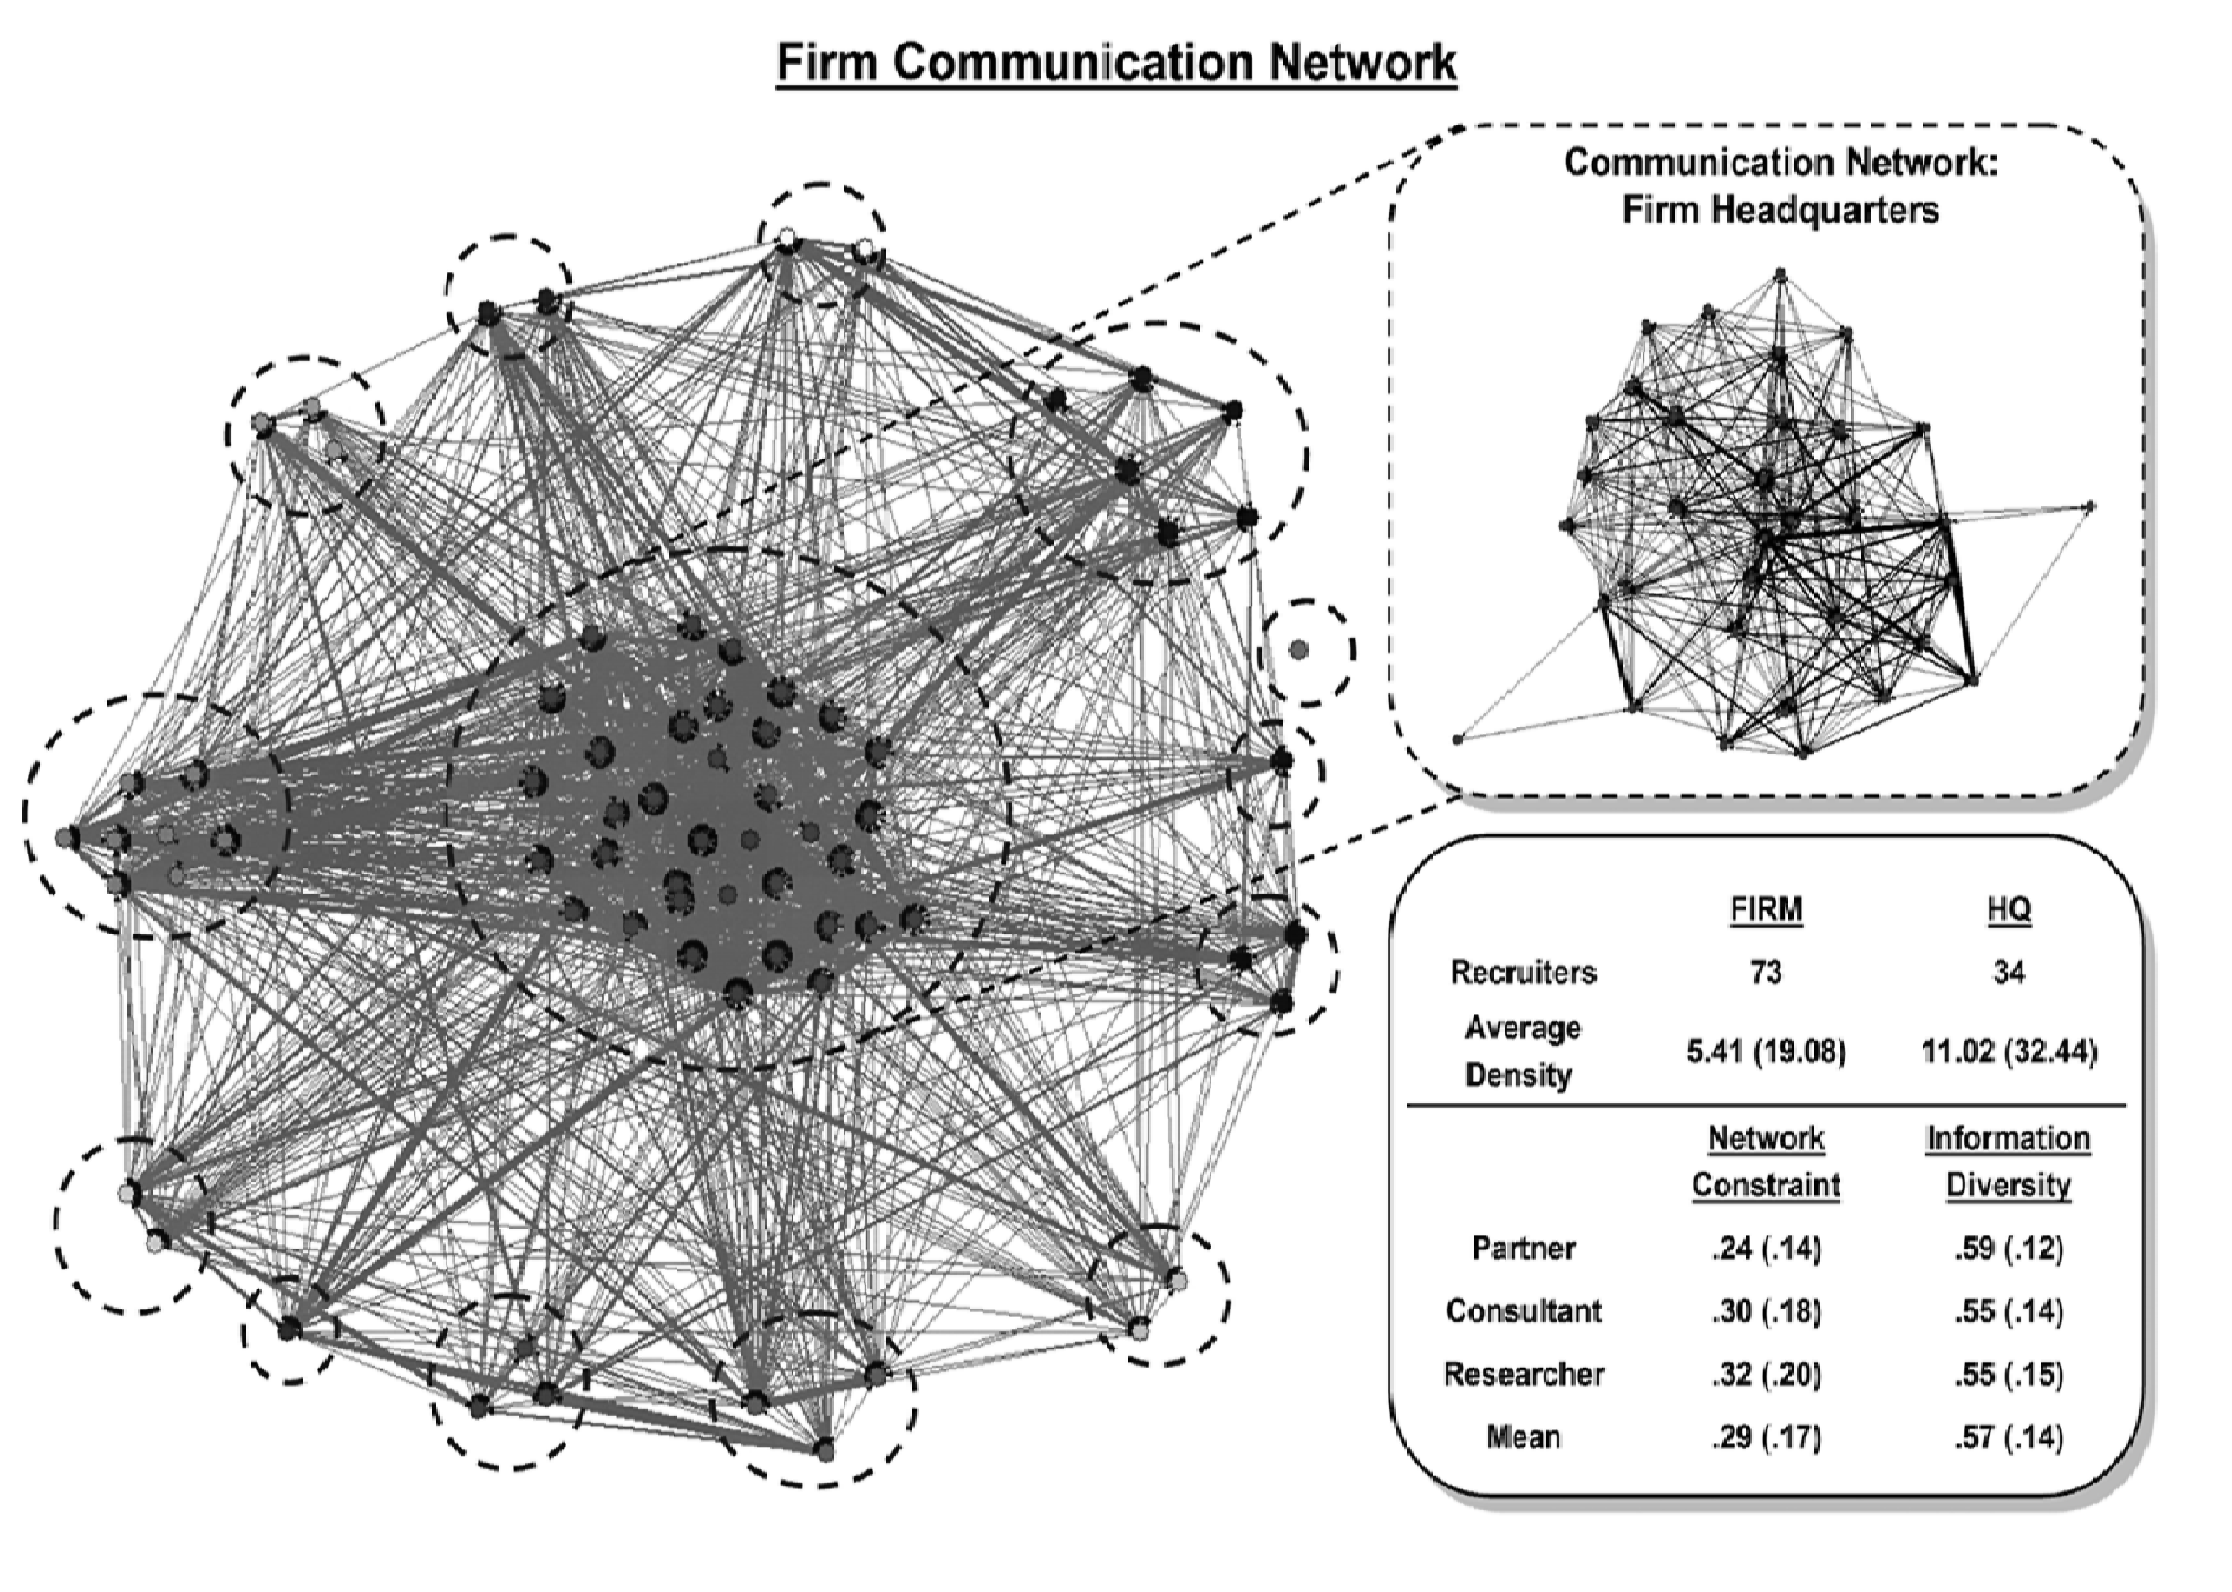
\includegraphics[width=\linewidth]{comm-net.png}
        % \caption{Cosine Distance}
      \end{figure}
    \end{column}
    
  \end{columns}

  \note{
    
  }

\end{frame}

\begin{frame}{{\color{violet}DVs: Recruiter Success Metrics}}

  \begin{itemize}
    \item Number of projects completed per month
    \item Revenues generated per month
    \item Average project duration (\~Productivity)
  \end{itemize}

  % \note{
    
  % }

\end{frame}
\begin{frame}{{\color{violet}IVs: Network Variables}}

  \begin{itemize}
    \item Network Size of Ego
    \item Network {\color{sred}Diversity} of Ego
    \begin{itemize}
      \item Structural Diversity
      \item Avg. Structural Equivalence of actors' contacts
    \end{itemize}
    \item Channel {\color{turq}Bandwidth} of Ego
  \end{itemize}

  % \note{
    
  % }

\end{frame}
\begin{frame}{{\color{violet}IVs: Information Diversity \& {\color{salmon}Novelty} -- Ego}}

  \begin{columns}

    \begin{column}{0.5\linewidth}
      \begin{itemize}
        \item Topic Vectors by Keyword
        \item Keyword Selection: $k$-means Clustering of topics
        \item Information Diversity (${ID}_i$)
        \item {\color{salmon}Non-Redundant} Information (${NRI}_i$): ${ID}_i$ times total incoming e-mail 
      \end{itemize}
    \end{column}

    \begin{column}{0.5\linewidth}
      \begin{figure}
        \centering
        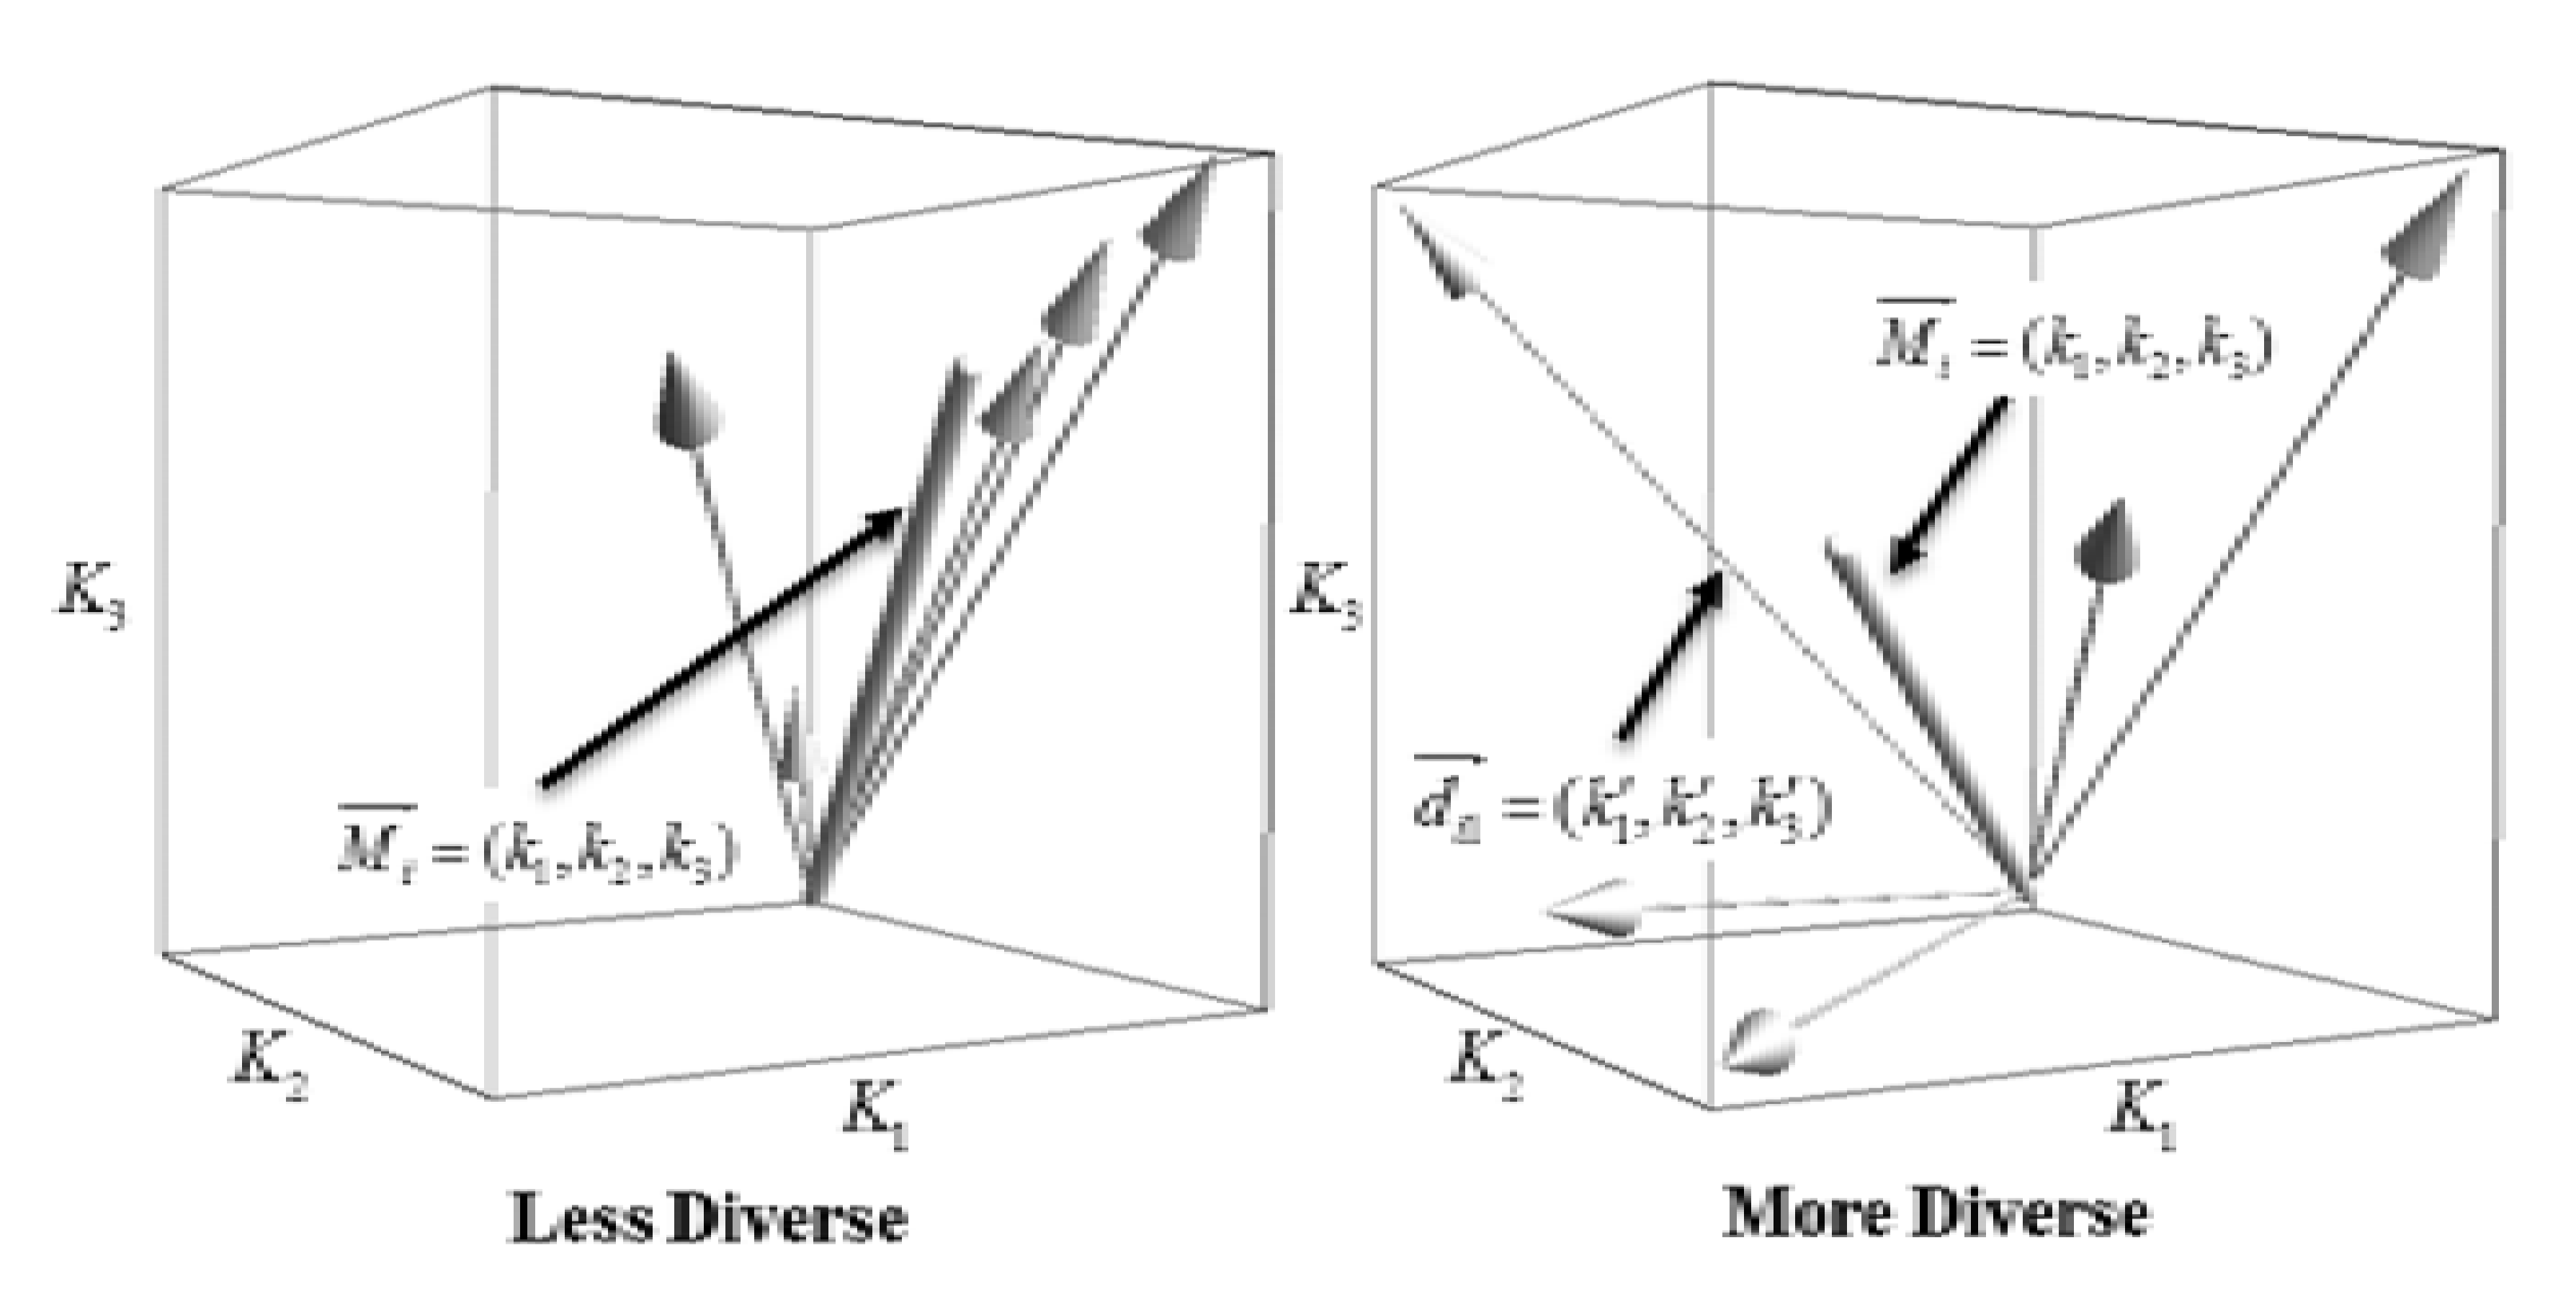
\includegraphics[width=\linewidth]{cos-dist2.png}
        % \caption{Cosine Distance}
      \end{figure}
      $${CosDist}_{ij} = 1 - Cos(d_{ij},M_{i})$$
      $${ID}_{i} = \frac{{\sum_{j=1}^{N} {CosDist}_{j}}^2}{N}$$
    \end{column}
    
  \end{columns}

  \note{
    k-means: High-frequency words in topics that maximize inter-topic coefficient of variation \& minimize intra-topic mean frequency variation.  
    ID: Avg. \underline{cosine distance} from \underline{cluster mean vector}
  }

\end{frame}

\begin{frame}{{\color{violet}IVs: Information Diversity \& {\color{salmon}Novelty} -- Ego}}

  \begin{columns}

    \begin{column}{0.5\linewidth}
      \begin{itemize}
        \item Topic Vectors by Keyword
        \item Keyword Selection: $k$-means Clustering of topics
        \item Information Diversity (${ID}_i$)
        \item {\color{salmon}Non-Redundant} Information (${NRI}_i$): ${ID}_i$ times total incoming e-mail 
      \end{itemize}
    \end{column}

    \begin{column}{0.5\linewidth}
      \begin{figure}
        \centering
        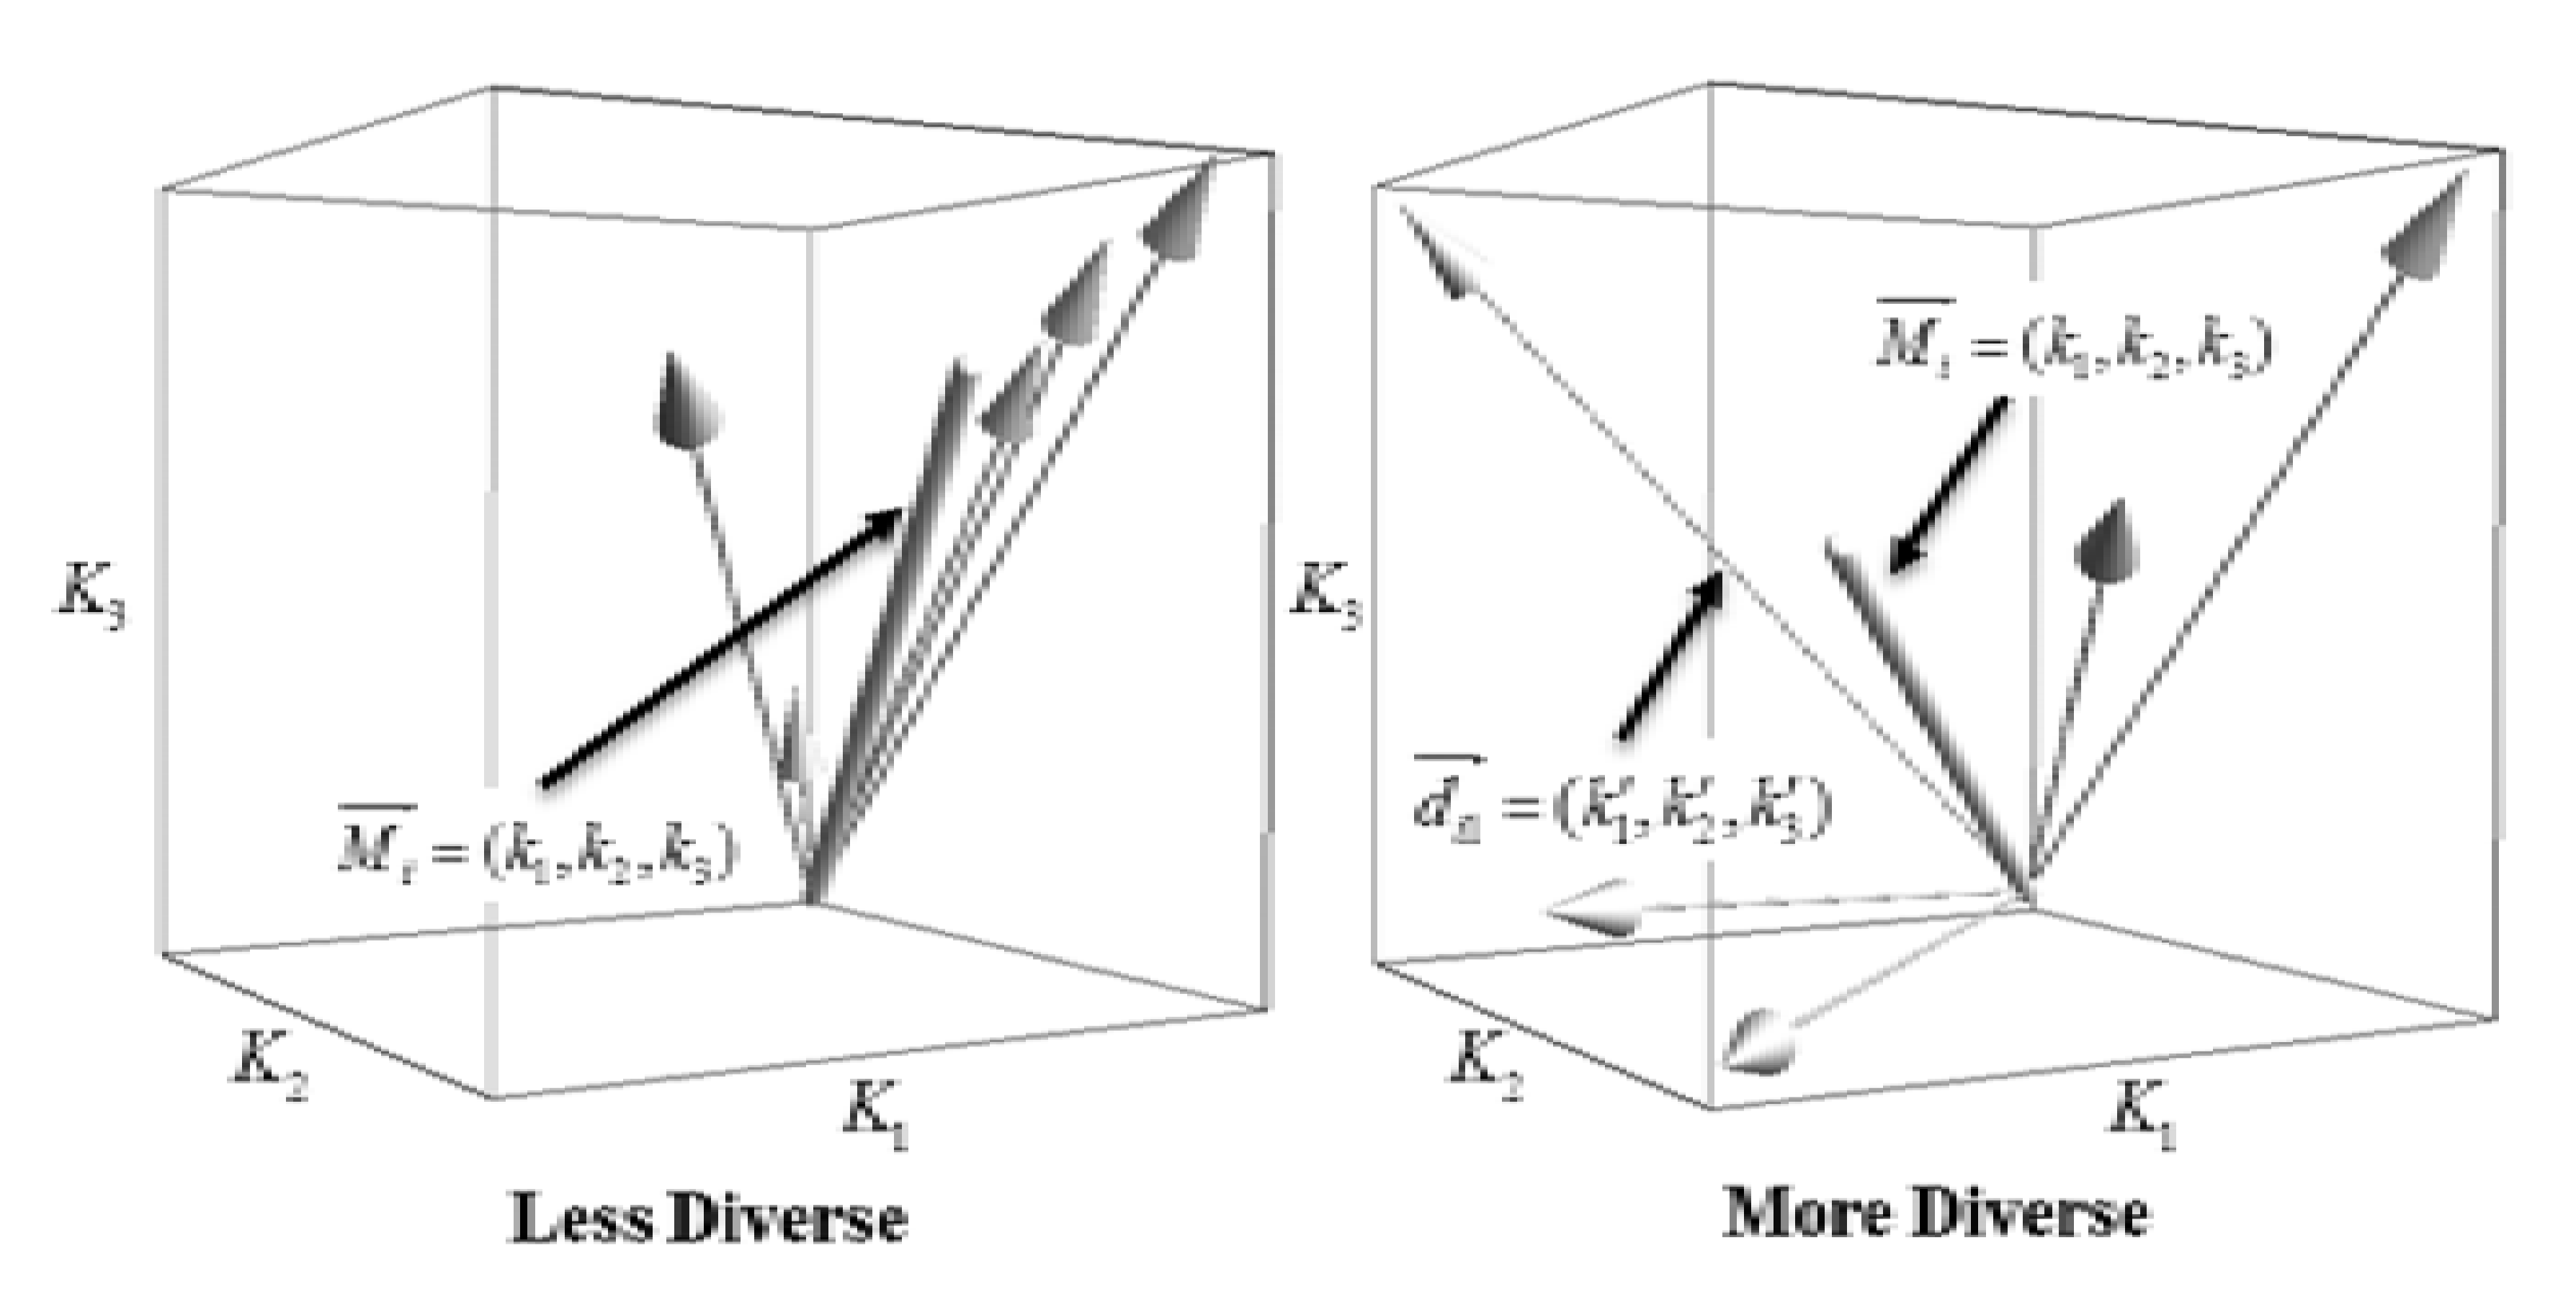
\includegraphics[width=\linewidth]{cos-dist2.png}
        % \caption{Cosine Distance}
      \end{figure}
      $${CosDist}_{ij} = 1 - Cos(d_{ij},M_{i})$$
      $${ID}_{i} = \frac{{\sum_{j=1}^{N} {CosDist}_{j}}^2}{N}$$
    \end{column}
    
  \end{columns}

  \note{
    k-means: High-frequency words in topics that maximize inter-topic coefficient of variation \& minimize intra-topic mean frequency variation.  
    ID: Avg. \underline{cosine distance} from \underline{cluster mean vector}
  }

\end{frame}

\begin{frame}{{\color{violet}IVs: Information Diversity \& {\color{salmon}Novelty} -- Alters}}

  \begin{itemize}
    \item Refresh-rate of alters: \underline{Cosine distance} between every forward pair of \underline{daily} e-mail vectors.
    \item Topic space of alters: Total {\color{salmon}non-redundant} information in ego's neighborhood.
    \item Information Overlap of alters: Total avg. {\color{salmon}redundant} information in ego's neighborhood
  \end{itemize}

\end{frame}

\begin{frame}{{\color{violet}IVs: Information Diversity \& {\color{salmon}Novelty} -- Alters}}

  \begin{itemize}
    \item Refresh-rate of alters: \underline{Cosine distance} between every forward pair of \underline{daily} e-mail vectors.
    \item Topic space of alters: Total {\color{salmon}non-redundant} information in ego's neighborhood.
    \item Information Overlap of alters: Total avg. {\color{salmon}redundant} information in ego's neighborhood
  \end{itemize}

\end{frame}

\begin{frame}{{\color{violet}IVs: Controls}}

  \begin{itemize}
    \item Expertise Heterogeneity of alters: \underline{Herfindahl index} of alters' expertise
    \item Demographic variables: Age and gender
    \item Human Capital: Level of education, No. of years in recruiting, Organizational position
    \item Total Communication volume
    \item Individual characteristics and Temporal shocks
  \end{itemize}

\end{frame}

% \begin{frame}{{\color{violet}IVs: Controls}}

  \begin{itemize}
    \item Expertise Heterogeneity of alters: \underline{Herfindahl index} of alters' expertise
    \item Demographic variables: Age and gender
    \item Human Capital: Level of education, No. of years in recruiting, Organizational position
    \item Total Communication volume
    \item Individual characteristics and Temporal shocks
  \end{itemize}

\end{frame}

\begin{frame}{{\color{violet}Model Specification}}

  \begin{itemize}
    \item Type 1: Fixed and Random-Effects models
    \begin{itemize}
    	\item To control for bias created by unobservable heterogeneity
    \end{itemize}
    \item Type 2: Network Auto-correlation model
    \begin{itemize}
    	\item Provides consistent estimates since network data are not independent
    \end{itemize}
  \end{itemize}

\end{frame}

\begin{frame}{{\color{violet}Concluding Comments}}

  \begin{itemize}
    \item Well-theorized Feature extraction from content
    \item Clean, testable generative mechanisms
    \item Validated construct choices with simulated data
    \item Probabilistic Topic Models instead of k-means?
    \item ERGMs?
  \end{itemize}

\end{frame}

\begin{frame}{{\color{violet}Questions}}

  \begin{figure}
    \centering
    
\includegraphics[width=\linewidth]{q1.png}
  \end{figure}

  \vspace{2ex}

  \begin{figure}
    \centering
    
\includegraphics[width=\linewidth]{q2.png}
  \end{figure}

\end{frame}



% \begin{frame}{A slide title}

  \begin{itemize}
    \item A bulleted item
    \item Another item
      \begin{itemize}
        \item With sub-bullets
        \item And another, with some \textbf{bold} text
      \end{itemize}
    \item And another, at the top level, with \textit{italic} text
  \end{itemize}

  \note{
    Here's a note for this slide.
  }

\end{frame}

% \begin{frame}{A 50-50 split slide}

  \begin{columns}

    \begin{column}{0.5\linewidth}
      \begin{itemize}
        \item This side has a bullet
        \item And another bullet, with text that wraps if it's long
      \end{itemize}
    \end{column}

    \begin{column}{0.5\linewidth}
      \begin{figure}
        \centering
        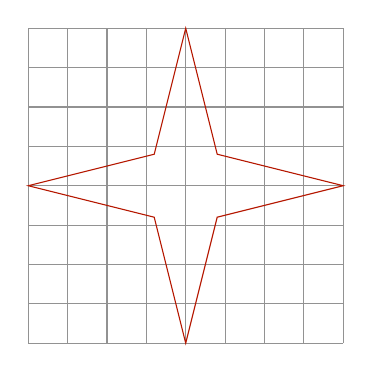
\begin{tikzpicture}[scale=2]
          \draw[step=0.25cm,color=gray] (-1,-1) grid (1,1);
          \draw[color=red] (1,0) -- (0.2,0.2) -- (0,1) -- (-0.2,0.2) -- (-1,0)
          -- (-0.2,-0.2) -- (0,-1) -- (0.2,-0.2) -- cycle;
        \end{tikzpicture}
        \caption{A figure caption}
      \end{figure}
    \end{column}
    
  \end{columns}

  \note{
    This slide has notes too.
  }

\end{frame}

% \begin{frame}{Full-slide figure}

  \begin{figure}
    \centering
    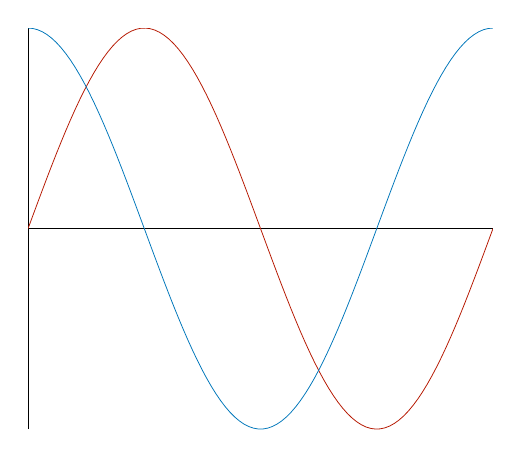
\begin{tikzpicture}[scale=0.7]
      \begin{axis}[
          scale only axis,
          no markers,
          domain=0:2*pi,
          samples=100,
          axis lines=center,
          axis line style={-},
          ticks=none]
        \addplot[red] {sin(deg(x))};
        \addplot[blue] {cos(deg(x))};
      \end{axis}
    \end{tikzpicture}
    \caption{The figure's caption}
  \end{figure}


\end{frame}

% \begin{frame}{A slide with centered text}

  \begin{center}
    Some statement that is centered.
  \end{center}

  \vspace{2ex}
  \begin{center}
    \scriptsize (a small note)
  \end{center}

\end{frame}

% \begin{frame}[fragile]{A slide with some code}

	\begin{columns}
		\begin{column}{0.5\linewidth}
			\footnotesize
			\begin{Verbatim}[commandchars=\\\{\}]
/* some code */
def foo(x):
  return x**0.5 + 2*x

\color{blue}/* some can be highlighted */
\color{blue}foo(3)
      \end{Verbatim}
    \end{column}
    \begin{column}{0.5\linewidth}
      {\color{red} Some explanatory text, in red, with some \texttt{monospace} text.}
      There might be some math, too:

      $$\sqrt{x} + 2x$$
    \end{column}
  \end{columns}

\end{frame}

% \begin{frame}{A slide with some bracketed text}

	\begin{itemize}
		\item Some statement {\color{gray} [Some citation]}
		\item Another statement {\color{gray} [Another citation]}
		\item A final statement {\color{gray} [The last citation]}
	\end{itemize}

	\vspace{3ex}
	\begin{center}
		\scriptsize (a small note)
	\end{center}

\end{frame}


% \begin{frame}{A slide with some text and a link}

  \begin{itemize}
    \item This slide has some text along with a link
      \begin{itemize}
        \item \textbf{Some bold text}: followed by an explanation
        \item \textbf{More bold text}: followed by more text
      \end{itemize}
    \item Another bullet, with sub-bullets
      \begin{itemize}
        \item A sub-bullet
        \item Another sub-bullet, with more text
      \end{itemize}
  \end{itemize}

  \vspace{2ex}
  \begin{center}
    \color{blue} \href{https://github.com/anishathalye/auriga}{github.com/anishathalye/auriga}
  \end{center}

\end{frame}


\end{document}
